\chapter{Testautomatisierung}
\label{sec:testautomatisierung}
In Kapitel \ref{sec:testautoGrundlagen} wurde der Begriff Testautomatisierung bereits eingeführt. Die darin dargelegte Definition hat gezeigt, dass man unter Testautomatisierung nicht nur das automatisierte Ausführen von Testfällen versteht.
Testautomatisierung ist in allen Bereichen des Entwicklungs- bzw. Testprozesses möglich.
\glqq Das Spektrum umfasst alle Tätigkeiten zur Überprüfung der Softwarequalität im Entwicklungsprozess, in den unterschiedlichen Entwicklungsphasen und Teststufen sowie die entsprechenden Aktivitäten von Entwicklern, Testern, Analytikern oder auch der in die Entwicklung eingebundenen Anwender. Die Grenzen der Automatisierung liegen darin, dass diese nur die manuellen Tätigkeiten eines Testers übernehmen kann, nicht aber die intellektuelle, krative und intuitive Dimension dieser Rolle.\grqq\ \cite[S.7]{seidl_basiswissen_2012} \\
Die intellektuelle Dimension ist vor allem in den frühen Phasen des Testprozesses gefordert. Diese Phasen sind maßgeblich für die spätere Qualität der einzelnen Testfälle. Testautomatisierung wird daher nie die Arbeit eines Testanalysten voll ersetzen können.\\
Um so weiter der Testprozess voranschreitet, um so praktischer werden auch die zu erledigenden Aufgaben. Das Potential für eine Automatisierung steigt also im Laufe des Testprozesses.
Fewster und Graham \cite[vgl. S.18]{fewster_software_1999} stellen diesen Zusammenhang in einer Grafik bildlich dar.  Abbildung \ref{fig:intellektuellVsPraktisch} greift diese Darstellung auf und passt sie auf den in Kapitel \ref{sec:testprozess} vorgestellten Testprozess an. Die verschiedenen Möglichkeiten der Testautomatisierung werden in Kapitel \ref{sec:bereiche_der_testautomatisierung} geklärt. Zunächst soll jedoch die Frage beantwortet werden, weshalb eine Automatisierung von Testfällen überhaupt sinnvoll ist.

\begin{figure}[htb]
  \centering  
  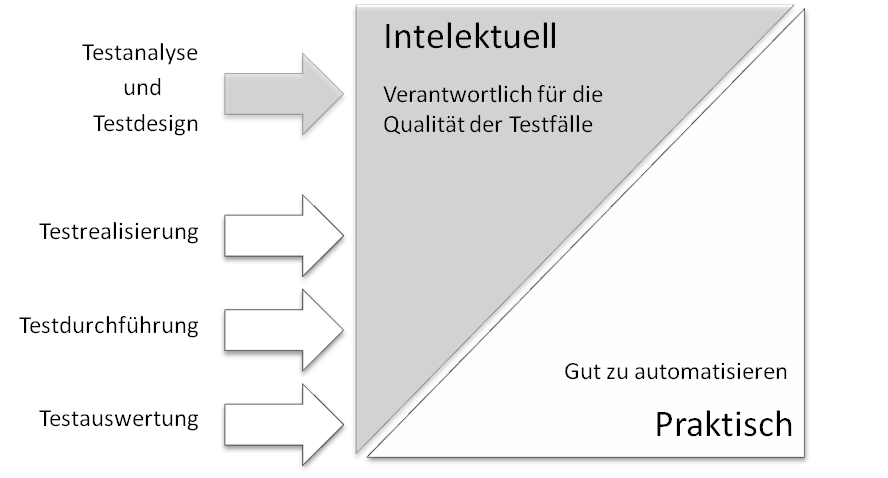
\includegraphics[scale=1]{img/intelektuellVsPraktisch.png}\\
  \footnotesize\sffamily\textbf{Quelle:} \cite[vgl. S.18]{fewster_software_1999}
  \caption{Grenzen und Möglichkeiten der Testautomatisierung}
  \label{fig:intellektuellVsPraktisch}
\end{figure}

\section{Warum Testautomatisierung}
\label{sec:warum_testautomatisierung}

Richtig durchgeführt kann Testautomatisierung eine Reihe von Vorteilen bringen. Dustin et al. \cite[S.44 ff.]{dustin_software_2001} stellen drei Hauptvorteile der Testautomatisierung fest:
\begin{itemize}
\item[1.] Erstellung eines zuverlässigen Systems
\item[2.] Verbesserung der Testqualität und Testtiefe
\item[3.] Verringerung des Testaufwands und Reduzierung des Zeitplans
\end{itemize}


In der Literatur gibt es zahlreiche Listen von Vorteilen der Testautomatisierung, die sehr viel feiner gegliedert sind, als die von Dustin et al. \cite[S.44 ff.]{dustin_software_2001} gewählten Oberpunkte.
So nennen beispielsweise Fewster und Graham \cite[vgl. S.9 ff.]{fewster_software_1999} oder auch Thaller \cite[vgl. S.28 ff.]{thaller_software-test_2002} eine Reihe von positiven Aspekten.\\
Gleicht man diese Vorteile mit den von Dustin et al. gewählten Oberpunkten ab, zeigt sich, dass vor allem die Verbesserung der Testqualität und Testtiefe (2), sowie die Verringerung des Testaufwands und die Reduzierung des Zeitplans (3), gut durch diese repräsentiert werden. Diese Oberpunkte lassen sich leicht mit den feiner ausformulierten Vorteilen unterfüttern.\\ Die Erstellung eines zuverlässigen Systems (1) ist hingegen nur schwer direkt durch feiner formulierte Vorteile zu untermauern. In der Regel wird dieser Punkt indirekt durch eine Verbesserung in den letzten beiden Bereichen (2,3) beeinflusst:\\
Eine Verringerung des Testaufwands für einzelne Tests schafft mehr Kapazität, die in bessere und breiter angelegte Tests investiert werden kann. Zusätzlich wird die Testqualität und Testtiefe direkt verbessert. Dies bedingt wiederum, dass mehr Fehler im System aufgedeckt werden können. Dadurch kann eine höhere Qualität des Endproduktes erreicht werden, die sich in einem zuverlässigeren System zeigt.\\
Da die Erstellung eines zuverlässigen Systems (1) nur schwer direkt durch feiner gegliederte Vorteile belegt werden kann und eher eine Folge der Verbesserung in den anderen beiden Bereichen (2,3) ist, wird sie im weiteren nicht näher betrachtet.\\
Fewster und Graham \cite[vgl. S.10]{fewster_software_1999} fassen die Vorteile der Testautomatisierung noch weiter zusammen und reduzieren sich in ihrem Fazit auf die Worte \grq Qualitäts- und Effizienzsteigerung\grq.
Diese Begriffe entsprechen weitestgehend den von Dustin et al. gewählten Oberpunkten. Qualitätssteigerung fasst dabei die Verbesserung der Testqualität und Testtiefe zusammen. Die Verringerung des Testaufwands und Reduzierung des Zeitplans entspricht der Effizienzsteigerung.\\
Um die Vorzüge der Testautomatisierung auf eine feinere und damit greifbarere Ebene zu bringen, werden im Folgenden die Vorteile, wie sie 
Fewster und Graham beschreiben, verwendet und den von Dustin et al. gewählten Oberpunkten zugeordnet.

\subsection{Verringerung des Testaufwands und Reduzierung des Zeitplans}
\label{sec:verringerung_des_testaufwands_und_reduzierung_des_zeitplans}
Die Vorteile in folgender Aufzählung nach Fewster und Graham \cite[vgl. S. 9 ff.]{fewster_software_1999} beschreiben, dass der Aufwand, der für das Testen einer Software betrieben werden muss, mit Hilfe von Automatisierung reduziert werden kann.
Reduzierter Aufwand in den Tests, sowie eine schnellere und wiederholbare Abarbeitung der Testfälle, führen dann meist dazu, dass der gesamte Zeitplan des Projekts positiv beeinflusst wird. Sein volles Potential entfaltet Automatisierung immer dann, wenn Testfälle wiederholt ausgeführt werden. Regressionstests, die vor jedem neuen Releasezyklus einer Software durchgeführt werden, sind daher prädestiniert dazu, automatisiert zu werden. Tester können so von sich wiederholenden Testaufgaben entlastet werden. Das reduziert den Testaufwand und stellt Tester für andere Aufgaben frei, was wiederum das gesamte Projekt beschleunigt.

\begin{itemize}
\item \textit{Ausführen existierender Regressionstests für eine neue Version der Software} \\
Der Aufwand, um Regressionstests manuell durchzuführen, kann schnell sehr groß werden. Sind Testfälle automatisiert, ist es möglich, sie bei Änderungen am System mit wenig Aufwand erneut durchzuführen.
\item \textit{Besserer Einsatz von Resourcen} \\
Mittels Automatisierung lässt es sich vermeiden, Tester durch generischen Aufgaben, wie beispielsweise das immer gleiche erzeugen von Testeingaben, zu binden.
Die frei gewordenen Resourcen können für andere Aufgaben verwendet werden.
Der Zeitplan des Projektes kann so verkürzt werden. 
\item \textit{Wiederverwendbarkeit von Testfällen} \\
Neue Projekte können von den Ergebnissen der Testautomatisierung aus vorangegangenen Projekten profitieren. Auch innerhalb eines Projektes können Teile von automatisierten Testfällen oftmals wiederverwendet werden.
Eine Reduzierung des Zeitplans ist dadurch möglich.
\item \textit{Frühere Markteinführung} \\
Richtig eingesetzt, beschleunigt Testautomatisierung den gesamten Testprozess. Das verkürzt letztendlich auch die Zeit bis zur Markteinführung des Softwareprodukts. 
\end{itemize}


\subsection{Verbesserung der Testqualität und Testtiefe}
\label{sec:verbesserung_der_testqualität_und_testtiefe}
Auch zeigen die beschriebenen Vorteile von Fewster und Graham \cite[vgl. S. 9 ff.]{fewster_software_1999}, dass sich mit Hilfe der Testautomatisierung Verbesserungen im Bereich der Testqualität und Testtiefe erreichen lassen. Eine bessere Testqualität wird meist dadurch erzielt, dass die Testfälle in ihrer Gesamtheit ein höheres Potential erreichen, Fehler aufzudecken. Vor allem eine höhere Testtiefe und eine breitere Testabdeckung sind hier die treibenden Faktoren. Auch die Qualität einzelner Testfälle kann mittels Testautomatisierung direkt verbessert werden. Eine bessere Wiederholbarkeit ist hier der maßgebende Faktor.


\begin{itemize}
\item \textit{Mehr Testfälle öfter ausführen} \\
Aus Zeitmangel müssen sich Tester oft auf einen geringeren Testumfang zurückziehen, als eigentlich gewünscht ist. Vor allem bei sehr generischen Testfällen, die sich beispielsweise nur in verschiedenen Maskeneingaben unterscheiden, ist es mit Hilfe von Testautomatisierung möglich, in weniger Zeit ein Vielfaches an Testfällen durchzuführen.
Eine tiefere Testabdeckung ist die Folge. Da solche Testfälle in der Regel auf einem zentralen Basistestfall beruhen, ist es hier besonders einfach möglich, eine durchgehend hohe Testqualität zu gewährleisten.
\item \textit{Testfälle durchführen, die ohne Automatisierung schwer bis unmöglich wären} \\
Einen Lasttest mit z.B. mehr als 200 Benutzern manuell durchzuführen, erweist sich als nahezu unmöglich. Die Eingaben von 200 Benutzern lassen sich mit Hilfe von automatisierten Lasttests jedoch gut simulieren. Über Testfälle, die ohne Automatisierung gar nicht möglich wären, lässt sich die Testbreite erhöhen. Die Qualität der Tests steigt durch das erhöhte Potential, Fehler zu entdecken.
\item \textit{Konsistenz und Wiederholbarkeit von Testfällen} \\
Testfälle, die automatisch durchgeführt werden, werden immer auf die gleiche Weise ausgeführt. Eine derartige Konsistenz ist auf manuellem Wege kaum zu erreichen. Fehler können somit vermieden und die Qualität gesteigert werden. 
\item \textit{Erhöhtes Vertrauen in die Testfälle und Software } \\
Das Wissen, dass eine Vielzahl an Testfällen erfolgreich vor jedem Release durchgeführt wurden, erhöht das Vertrauen von Entwickler und Nutzern, dass unerwartete Fehler ausbleiben.
Werden Testfälle regelmäßig ausgeführt, erhöht das zusätzlich das Vertrauen, dass diese Testfälle stabil sind und keine Falschmeldungen auftreten.
\end{itemize}


\subsection{Kosten als Bewertungsgrundlage für die Testautomatisierung}
\label{sec:kosten_der_testautomatisierung}
Die unter Kapitel \ref{sec:verbesserung_der_testqualität_und_testtiefe} und Kapitel \ref{sec:verringerung_des_testaufwands_und_reduzierung_des_zeitplans} aufgezeigten Vorteile der Testautomatisierung haben das Problem, dass sie sich meist nur schwer messen und mit genauen Zahlen belegen lassen.
Um das zu erreichen, muss man sich auf die kleinste gemeinsame Größe berufen, auf die all die genannten Vorteile hinarbeiten: Eine Kostenreduzierung beim Testen.
Sowohl eine Verbesserung der Testqualität und Testtiefe, als auch eine Verringerung des Testaufwands und Reduzierung des Zeitplans, verfolgen in letzter Instanz immer das Ziel, Kosten einzusparen.\\
Um den Nutzen der Testautomatisierung für ein Projekt messbar zu machen und nachvollziehbar zu begründen, bieten nach Ramler und Wolfmaier \cite{ramler_economic_2006} daher die direkten Kosten, die durch das Erstellen und Ausführen der Testfälle entstehen, den besten Ansatzpunkt. 
Ramler und Wolfmaier \cite{ramler_economic_2006} zitieren eine Fallstudie von Linz und Daigl \cite{dustin_automated_1999}, die eine Unterteilung der Kosten in zwei Komponenten vornimmt.
\begin{itemize}
    \item[] \(V:=\text{Ausgaben für Testspezifikation und Implementierung}\)
    \item[] \(D:=\text{Ausgaben für einen einzelnen Testlauf}\)
\end{itemize}

Mit Hilfe dieser beiden Variablen können die Kosten (\(A_a\)) für einen einzelnen automatisierten Testfall wie folgt angegeben werden:
\begin{equation}
A_a:=V_a+n*D_a
\end{equation}
\(V_a\) symbolisiert die Kosten, die für die Spezifikation und Implementierung des automatisierten Testfalls anfallen. \(D_a\) die Kosten, die für das einmalige Ausführen des Testfalles entstehen und \(n\) steht für die Anzahl der durchgeführten Testläufe.
Um zu bestimmen, wie sich das manuelle und automatisierte Testen zueinander verhalten, kann analog die selbe Gleichung für das manuelle Testen aufgestellt werden.
\begin{equation}
A_m:=V_m+n*D_m
\end{equation}

Mit Hilfe dieser beiden Gleichungen lässt sich zeigen, dass sich ab einer gewissen Anzahl an Testläufen, die Automatisierung gegenüber der manuellen Ausführung, bezüglich der Kosten lohnt.
Es wird dabei davon ausgegangen, dass die initiale Investition \(V_a\) für die Automatisierung höher ist, als die initiale Investition für das manuelle Testen \(V_m\).
Die Kosten \(A_a\) des automatisierten Testfalls steigen mit jeder Testausführung \(n\) jedoch langsamer an. Beide Funktionen schneiden sich daher in einem Break-Even-Point, ab dem die Automatisierung die günstigere Alternative darstellt.
Abbildung \ref{fig:breakEven} veranschaulicht diesen Zusammenhang grafisch.

\begin{figure}[htb]
  \centering  
  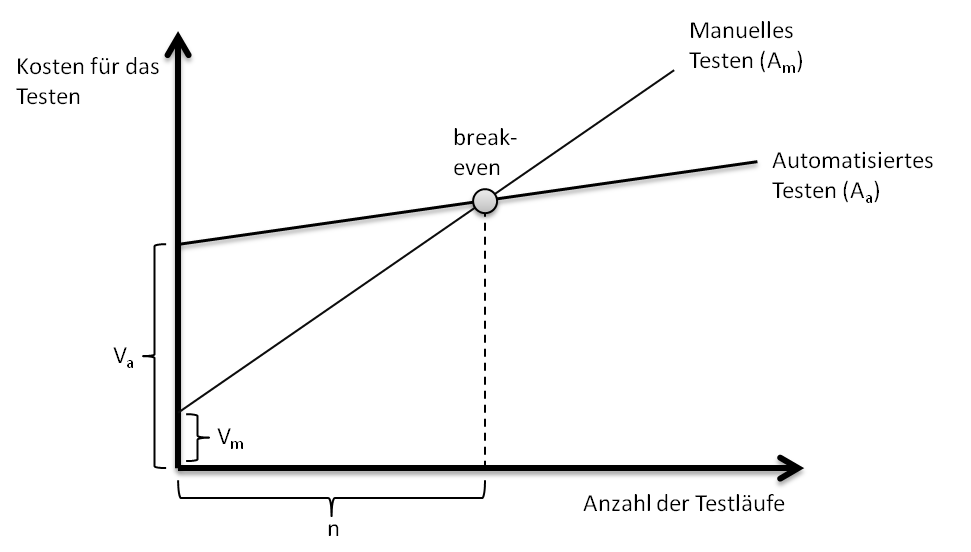
\includegraphics[scale=0.8]{img/breakeven.png}\\
  \footnotesize\sffamily\textbf{Quelle:} \cite{ramler_economic_2006}
  \caption{Break-Even-Point für Testautomatisierung}
  \label{fig:breakEven}
\end{figure}

Zusammenfassend lässt sich feststellen, dass vor allem wiederholt ausgeführte Testtätigkeiten hohes Einsparungspotential bei einer Testautomatisierung bieten.


\subsection{Probleme der Testautomatisierung}
\label{sec:probleme_der_testautomatisierung}
Ramler und Wolfmaier \cite{ramler_economic_2006} zitieren ein Erreichen des Break-Even-Point, wie er in Kapitel \ref{sec:kosten_der_testautomatisierung} beschrieben ist, nach einer Ausführung von 2-20 Testläufen. Diese große Spanne macht deutlich, wie wichtig es ist, in der Testplanung und Steuerung genau abzuwägen, ob und wo eine Automatisierung sinnvoll einzusetzen ist. Eine Automatisierung kann oft auch unwirtschaftlich sein, vor allem immer dann, wenn Tests nur ein einziges mal ausgeführt werden. Implementierungs- und Wartungsaufwand von automatisierten Testfällen sind meist sehr viel höher, als der von manuellen Testfällen. Dieser Mehraufwand muss in irgend einer Weise gerechtfertigt sein. Laut Fewster und Graham \cite[vgl. S. 22 ff.]{fewster_software_1999} und auch Thaller \cite[vgl. S.230 ff.]{thaller_software-test_2002} wird dieser Punkt oftmals vernachlässigt und die Testautomatisierung als Heilmittel für schlecht laufende Prozesse und zu hohe Kosten gesehen. Dabei ist genau das Gegenteil der Fall. Es ist sinnvoller, zunächst die Qualität der Tests und des eigenen Testprozesses zu optimieren, bevor eine Automatisierung eingeführt wird.\\ 
Ein weiterer Schwachpunkt der Automatisierung ist nach Fewster und Graham \cite[vgl. S. 22 ff.]{fewster_software_1999}, dass die Automatisierung von Software-Tests zwar einen Mehraufwand bedeutet, jedoch die Anzahl der gefundenen Fehler nur geringfügig erhöht wird.
Bevor Testfälle automatisiert werden, müssen sie in der Regel zuvor einmal manuell durchgeführt werden, um sicher zu stellen, dass der angedachte Test auch sinnvoll und realisierbar ist. Meist werden Fehler bereits bei dieser manuellen Überprüfung festgestellt. Wird der Testfall dann automatisiert, deckt er weit weniger wahrscheinlich einen Fehler auf, als bei seiner ersten, manuellen Ausführung. Darüber hinaus können automatisierte Testfälle Fehler nur über die Akzeptanzkriterien aufdecken, die ihnen explizit hinterlegt wurden. Oft reichen die hinterlegten Kriterien aber nicht aus, um alle Fehlerquellen abzudecken. Das kann laut Fewster und Graham \cite[vgl. S. 23 ff.]{fewster_software_1999} dazu führen, dass Testfälle als positiv gekennzeichnet werden, obwohl sie in Wirklichkeit fehlerhaft waren. Bei manuellen Tests fallen vergessene Akzeptanzkriterien eher auf bzw. werden durch den Tester intuitiv ergänzt. Die Anzahl der fälschlicherweise positiv gewerteten Testfälle sinkt also mit der manuellen Durchführung.\\
Einen weiteren positiven Aspekt, den Fewster und Graham \cite[vgl. S. 24 ff.]{fewster_software_1999} in einem manuellen Tester sehen, ist eine höhere Stabilität in den Testfällen. Ein Tester kann sich auf kleinere Änderungen in der zu testenden Software leicht einstellen. Er kann selbst entscheiden, ob eine Abweichung vom Testfall als Fehler zu werten oder zu vernachlässigen ist. Automatisierte Testfälle bieten diesen Luxus nicht. Sie verfolgen einen festen Ablaufplan und können nur schwer mit Veränderungen in der zu testenden Software umgehen. Das macht sie, im Vergleich zu manuellen Tests, instabil und erfordert einen erhöhten Wartungsaufwand. In manchen Fällen kann diese Abhängigkeit zwischen Software und automatisiertem Test sogar so weit führen, dass sie die Entwicklung der Software behindern. Beispielsweise dann, wenn eine Änderung so große Auswirkungen auf die automatisierten Testfälle hätte, dass es aus wirtschaftlicher Sicht nicht mehr sinnvoll ist sie durchzuführen. Die Kosten für die Anpassungen wären dann so hoch, dass sie den Nutzen der Softwareänderung übersteigt.\\
Analog zu den in Kapitel \ref{sec:verringerung_des_testaufwands_und_reduzierung_des_zeitplans} und \ref{sec:verbesserung_der_testqualität_und_testtiefe} genannten Vorteilen haben Fewster und Graham \cite[vgl. S. 10 ff.]{fewster_software_1999} auch eine Liste mit bekannten Nachteilen der Testautomatisierung aufgestellt, welche die gerade angesprochenen Probleme noch einmal aufgreifen und ergänzen:

\begin{itemize}
\item \textit{Unrealistische Erwartungen} \\
Testautomatisierung wird oft als Lösung für alle Testprobleme gesehen. Es ist wichtig, dass die Erwartungen aller Beteiligten realistisch bleiben.
\item \textit{Schlechte Testpraxis } \\
Wenn das Testen in einem Unternehmen bereits eine Schwachstelle darstellt, ist es nicht sinnvoll eine Testautomatisierung einzuführen. Es ist besser, zunächst die vorherrschenden Prozesse zu optimieren.
\item \textit{Die Anzahl der gefundenen Fehler wird sich nicht stark verändern } \\
Fehler werden meist bei der ersten Durchführung eines Testfalls aufgedeckt. Wird ein Testfall wiederholt, sinkt auch sein Potential Fehler aufzudecken. In der Regel werden Fehler bereits beim Entwickeln der automatisierten Testfälle entdeckt, nicht erst bei weiteren Testläufen.
\item \textit{Trügerische Sicherheit} \\
Die Tatsache, dass alle automatisierten Testfälle positiv waren bedeutet nicht, dass die Software auch frei von Fehlern ist. Möglicherweise sind nicht alle Bereiche der Software mit Testfällen abgedeckt oder die Akzeptanzkriterien der Testfälle sind nicht umfassend genug gewählt worden. Auch ist es möglich, dass die Testfälle fehlerhaft sind und falsche Ergebnisse anzeigen.
\item \textit{Wartung} \\
 Automatisierte Testfälle haben einen hohen Wartungsaufwand. Änderungen an der Software bedingen oft auch, dass die Testfälle überarbeitet werden müssen. Wird dieser Wartungsaufwand so hoch, dass es günstiger wäre die Testfälle manuell durchzuführen, werden die automatisierten Tests unwirtschaftlich.
\item \textit{Technische Probleme} \\
Die Automatisierung von Testfällen stellt eine komplexe Aufgabe dar und ist daher oft mit Problemen verbunden. Die verwendeten Tools bzw. Frameworks sind meist selbst nicht befreit von Fehlern. Oft gibt es auch technische Probleme mit der zu testenden Software selbst.
\item \textit{Probleme in der Organisation} \\
Eine erfolgreiche Testautomatisierung stellt hohe Anforderungen an die technischen Fähigkeiten der Entwickler und erfordert starken Rückhalt in der Führungsebene. Testautomatisierung läuft nicht immer sofort reibungslos und benötigt oft Anpassungen in vorherrschenden Prozessen.
\end{itemize}


\section{Möglichkeiten der Testautomatisierung im Testprozess}
\label{sec:bereiche_der_testautomatisierung}
Wie bereits zu Beginn dieses Kapitels erwähnt, beschränkt sich die Testautomatisierung nicht nur auf das automatisierte Ausführen von Testfällen, sondern erstreckt sich über den gesamten Testprozess. Innerhalb des Testprozesses haben Amannejad et al. \cite{amannejad_search-based_2014} vier Hauptaufgaben identifiziert, die aus Sicht der Testautomatisierung besonders interessant sind:

\begin{itemize}
\item Testdesign: Erstellen einer Liste von Testfällen.
\item Testcodeerstellung: Erstellen von automatisiertem Testcode.
\item Testdurchführung: Ausführen von Testfällen und Aufzeichnen der Ergebnisse.
\item Testauswertung: Auswerten der Testergebnisse.
\end{itemize}

\subsection{Testdesign}
\label{subsec:testdesign}
Beim Testdesign handelt es sich um eine Aufgabe die laut Thaller \cite[vgl. S. 231]{thaller_software-test_2002} nicht unbedingt prädestiniert dafür ist, automatisiert zu werden. Abbildung \ref{fig:intellektuellVsPraktisch} hat bereits gezeigt, dass es sich um eine eher intellektuell geprägte Aufgabe handelt.
Dennoch gibt es eine Reihe von Möglichkeiten, wie das Entwerfen von Testfällen automatisiert werden kann. Die verschiedenen Ansätze beschränken sich in der Regel darauf, unterschiedliche Testeingaben für die zu testende Software zu finden.
Ein großes Problem, welches die Tools zum Entwerfen der Testfälle laut Fewster und Graham \cite[vgl. S. 19]{fewster_software_1999} dabei haben ist, dass sie einem fest vorgegebenem Algorithmus folgen. Dieses Vorgehen wird jedoch der intellektuellen Komponente dieser Aufgabe nicht gerecht. Ein Tester kann ähnlich strukturierte Testfallerstellungsmethoden heranziehen, wie sie beim automatisierten Testdesign verwendet werden. Um eine komplexe Software umfassend zu testen, reicht es jedoch meist nicht aus, einem festen Algorithmus nachzugehen. Eine tiefere Analyse durch einen Tester wird benötigt. Dieser ist in der Lage, außerhalb eines vorgegebenen Algorithmus, Testfälle zu identifizieren, fehlende Anforderungen zu finden oder sogar, aufgrund von persönlicher Erfahrung, Fehler in der Spezifikation aufzudecken.\\
Ein weiteres Problem das Fewster und Graham \cite[vgl. S. 19]{fewster_software_1999} nennen, ist die Menge an Testfällen, die mit Hilfe von automatisierten Methoden erzeugt werden. Die Anzahl der Testfälle kann schnell so groß werden, dass sie nicht mehr in einem vertretbarem Zeitaufwand durchgeführt werden können. In diesem Fall müssen aus der Menge an Testfällen, die wichtigsten identifiziert werden. Testfälle nach ihrer Relevanz zu filtern ist wiederum eine intellektuelle Aufgabe, die nur schwer in einem Automatisierungstool abgebildet werden kann.\\
Trotz ihrer Probleme haben Methoden zum automatisierten Testfalldesign durchaus ihre Daseinsberechtigung. Sie können die Arbeit des Testers beschleunigen, indem sie ihm einen Grundstock an Testfällen an die Hand geben, der durch weitere Testfälle erweitert werden kann. Sinnvoll ist es, sich nicht ausschließlich auf die Möglichkeit des automatisierten Testfalldesigns zu stützen, sondern sie mit den Fähigkeiten eines Tester zu kombinieren.\\
Seidel et al. \cite[vgl. S. 27]{seidl_basiswissen_2012} beschreiben eine Reihe an Testfallentwurfsmethoden, die sie unter dem Oberbegriff der Kombinatorik zusammenfassen. Diese Entwurfsmethoden zielen darauf ab, aus einer Fülle von möglichen Eingaben diejenigen herauszufiltern, die ein hohes Fehlerpotenzial in sich bergen. Darunter fallen beispielsweise:
\begin{itemize}
\item Äquivalenzklassenbildung
\item Grenzwertanalyse
\item Klassifikationsbaummethode
\end{itemize}
Diese Entwurfsmethoden kommen vor allem beim manuellen Designen von Testfällen zum Einsatz, bieten aber auch die Möglichkeit toolgestützt und damit automatisiert abzulaufen.
Fewster und Graham \cite[vgl. S. 19 ff.]{fewster_software_1999} beschreiben eine Reihe von weiteren Methoden zum Erzeugen von Eingabedaten, die vermehrt in automatisierten Tools zum Einsatz kommen:
\begin{itemize}
\item Codebasierte Generierung von Eingabedaten
\item Interfacebasierte Generierung von Eingabedaten
\item Spezifikationsbasierte Generierung von Eingabedaten
\end{itemize}

\subsubsection{Codebasierte Generierung von Eingabedaten}
\label{subsubsec:codebasierte_generierung}
Die Generierung der Eingabedaten erfolgt bei diesem Ansatz anhand der Struktur des Codes (siehe Abbildung \ref{fig:codeBasedDesign}). Jede Eingabe bedingt einen fest vorbestimmten Ablauf durch das Programm. Anhand des Codes können daher die benötigten Eingaben ermittelt werden, die für das durchlaufen von unterschiedlichen Pfaden im Programm benötigt werden.
Fewster und Graham \cite[vgl. S. 19 ff.]{fewster_software_1999} sehen in diesem Ansatz jedoch Probleme. Ein Testfall benötigt immer auch ein erwartetes Ergebnis. Über die Codebasierte Generierung ist es nicht möglich diese Ergebnisse zu ermitteln. Die generierten Testfälle sind also unvollständig.\\
Ein weiteres Problem dieses Vorgehens ist, dass ausschließlich der Code getestet wird, der bereits implementiert wurde. Fehlende Funktionalitäten können so nicht erkannt werden. Es wird getestet, dass der Code das \grq tut, was er tut und nicht das, was er tun soll.\grq\ \cite[vgl. S. 20]{fewster_software_1999}
\begin{figure}[htb]
  \centering  
  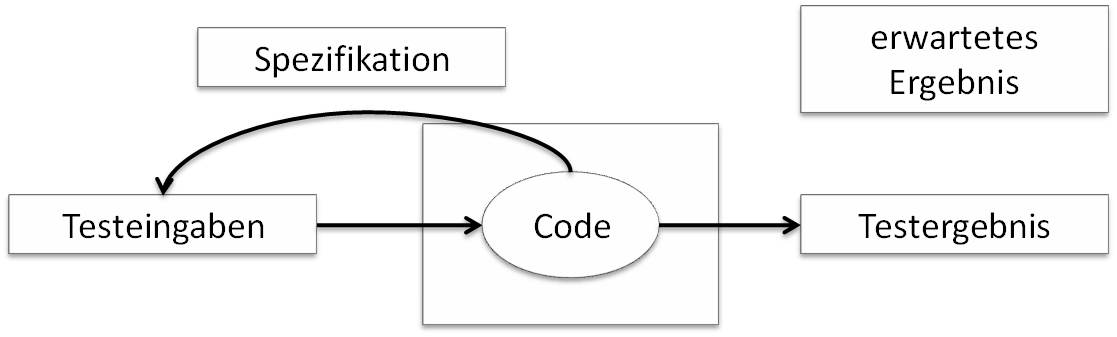
\includegraphics[scale=0.6]{img/codeBasedDesign.png}\\
  \footnotesize\sffamily\textbf{Quelle:} \cite[vgl. S. 19]{fewster_software_1999}
  \caption{Codebasierte Generierung von Testfällen}
  \label{fig:codeBasedDesign}
\end{figure}


\subsubsection{Interfacebasierte Generierung von Eingabedaten}
\label{subsubsec:interfacebasierte_generierung}
Bei dieser Methode erfolgt nach Fewster und Graham \cite[vgl. S. 20]{fewster_software_1999} die Generierung anhand von gut definierten Schnittstellen, wie der Benutzeroberfläche einer Desktop- oder Web-Anwendung (siehe Abbildung \ref{fig:interfaceBasedDesign}). 
Wird als Schnittstelle die Benutzeroberfläche gewählt, kann beispielsweise getestet werden, ob eine Checkbox nach einer Interaktion aktiviert bzw. deaktiviert wurde.\\
Eine weitere Möglichkeit wäre es, rekursiv jeden Link in einer Webanwendung zu durchlaufen. Alle defekten Links der Anwendung könnten auf diese Weise identifiziert werden.\\
Mit Hilfe dieses Ansatzes ist es laut Fewster und Graham \cite[vgl. S. 21]{fewster_software_1999} auch möglich, einfache Akzeptanzkriterien zu generieren. Werden beispielsweise die Links einer Web-Anwendung rekursiv durchlaufen, könnte als Akzeptanzkriterium geprüft werden, ob nach dem ausführen eines Links auch eine neue Webseite geladen wurde.

\begin{figure}[htb]
  \centering  
  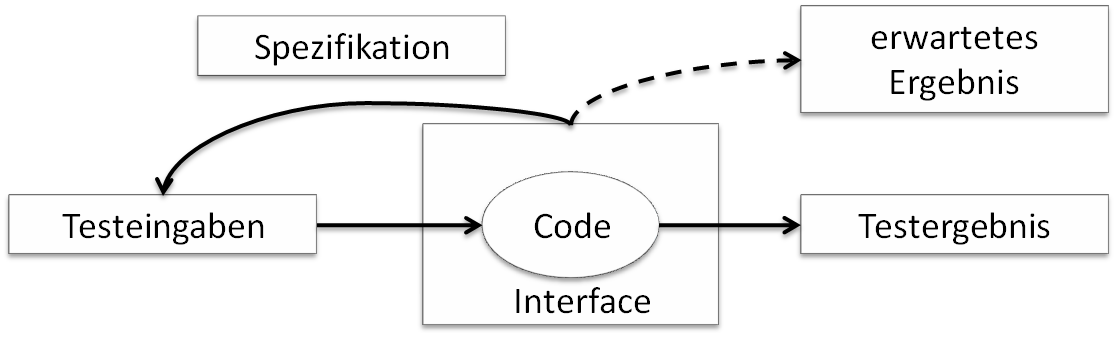
\includegraphics[scale=0.6]{img/interfaceBasedDesign.png}\\
  \footnotesize\sffamily\textbf{Quelle:} \cite[vgl. S. 20]{fewster_software_1999}
  \caption{Interfacebasierte Generierung von Testfällen}
  \label{fig:interfaceBasedDesign}
\end{figure}


\subsubsection{Spezifikationsbasierte Generierung von Eingabedaten}
\label{subsubsec:spezifikationsbasierte_generierung}
Mit Hilfe von Spezifikationsbasierter Generierung ist es nach Fewster und Graham \cite[vgl. S. 21]{fewster_software_1999} möglich sowohl Testeingaben, als auch die zugehörigen erwarteten Ergebnisse zu erzeugen (siehe Abbildung \ref{fig:specBasedDesign}). Als Basis wird dazu eine Spezifikation benötigt, die automatisiert analysiert werden kann. Die Möglichkeiten dafür reichen von natürlicher Sprache, die gewissen Strukturen folgt, bis hin zu technischen Modellen.\\ Vor allem die Benutzung von Modellen hat in den letzten Jahren immer mehr an Bedeutung gewonnen und ist heute unter dem Namen \grq modellbasiertes Testen\grq\ bekannt. Als Referenz auf diesem Gebiet kann das Werk von Roßner et al.\ \cite{rossner_basiswissen_2010}, \grq Basiswissen Modellbsierter Test\grq, dienen.\\
Ein Vorteil des Spezifikationsbasierten Ansatzes ist nach Fewster und Graham \cite[vgl. S. 21]{fewster_software_1999} auch, dass die Testfälle nicht auf Basis einer Implementierung, sondern auf Basis einer Spezifikation erzeugt werden. Damit wird sichergestellt, dass sie nicht nur, wie bei der Codebasierten Generierung, überprüfen \grq was die Software tut\grq , sondern \grq was die Software tun soll\grq.

\begin{figure}[htb]
  \centering  
  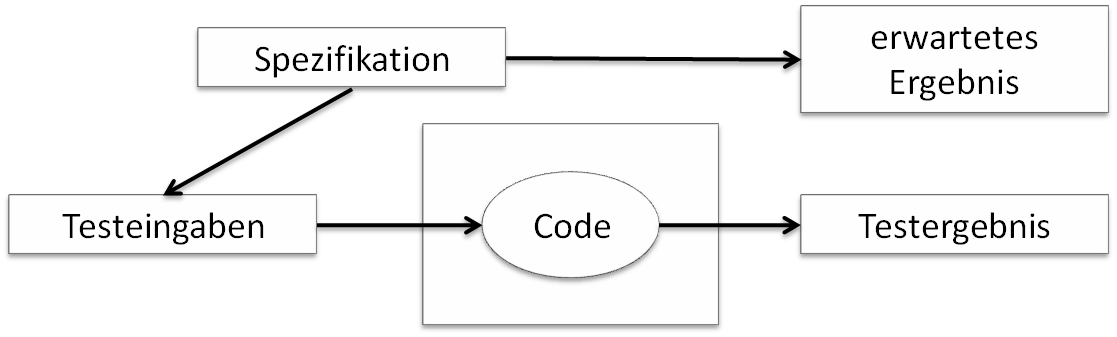
\includegraphics[scale=0.6]{img/specBasedDesign.png}\\
  \footnotesize\sffamily\textbf{Quelle:} \cite[vgl. S. 21]{fewster_software_1999}
  \caption{Spezifikationsbasierte Generierung von Testfällen}
  \label{fig:specBasedDesign}
\end{figure}

\subsection{Testcodeerstellung}
\label{subsec:testcodeerstellung}
Bei der Testautomatisierung versteht man unter Testcodeerstellung das Erzeugen von Testcode, der später wiederholt gestartet werden kann. Der erzeugte Code setzt die Testfälle um, die zuvor in der Designphase erarbeitet wurden.
In vielen Fällen handelt es sich hierbei um einen manuellen Schritt. Die Testcodeerstellung ist oft eine reine Entwicklertätigkeit, bei der ein Tester die angedachten Testfälle als Testcode implementiert.
Aber auch in diesem Schritt sind laut Amannejad et al. \cite{amannejad_search-based_2014} Möglichkeiten für eine Automatisierung gegeben.\\
Es existieren beispielsweise teilautomatisierte Ansätze. Mit Hilfe von sogenannten \grq record and playback\grq-Tools (R\&PB) können die Interaktionen eines Benutzers mit der zu testenden Software aufgezeichnet werden. Die aufgezeichneten Abläufe können dann verwendet werden, um automatisierte Testskripte zu generieren.\\
Auch ein vollautomatisierter Ansatz ist möglich, wenn auch nicht so weit verbreitet, wie der manuelle bzw. teilautomatisierte Ansatz.
Mittels modellbasiertem Testen ist es nicht nur möglich, wie in Kapitel \ref{subsubsec:spezifikationsbasierte_generierung} angesprochen, Testfalldesigns abzuleiten. Liegen die Modelle in einem entsprechend hohen Detailgrad vor, kann daraus sogar direkt Testcode erzeugt werden. Bouquet et al. \cite{bouquet_test_2008} beschreiben beispielsweise einen modellbasierten Ansatz, mit dessen Hilfe das Designen, Erstellen und Ausführen von Testfällen automatisiert geschehen kann.\\
Zusammengefasst ist die Testcodeerstellung damit in drei unterschiedlichen Automatisierungsgraden möglich:
\begin{itemize}
\item Manuell
\item Teilautomatisiert (R\&PB)
\item Automatisiert
\end{itemize}

Allen Ansätzen gemeinsam ist, dass sie immer eine Schnittstelle zum System benötigen, über welche der automatisierte Testcode mit der zu testenden Anwendung kommunizieren kann.
Meszaros et al. \cite{meszaros_agile_2003} unterscheiden dabei zwei Hauptangriffspunkte:
\begin{itemize}
\item API (application programming interface): Als Schnittstelle wird der Code der zu testenden Anwendung direkt benutzt.
\item UI (user interface): Als Schnittstelle wird die Benutzeroberfläche der Anwendung verwendet.
\end{itemize}

Kombiniert man die verschiedenen Ansätze der Testcodeerstellung mit den Schnittstellen, ergibt sich eine Matrix, welche die verschiedenen Möglichkeiten der Testcodeerstellung beim automatisierten Testen abbildet. Eine grafische Darstellung dieser Matrix bietet Abbildung \ref{fig:bereicheTestcodeerstellung}.


\begin{figure}[htb]
  \centering  
  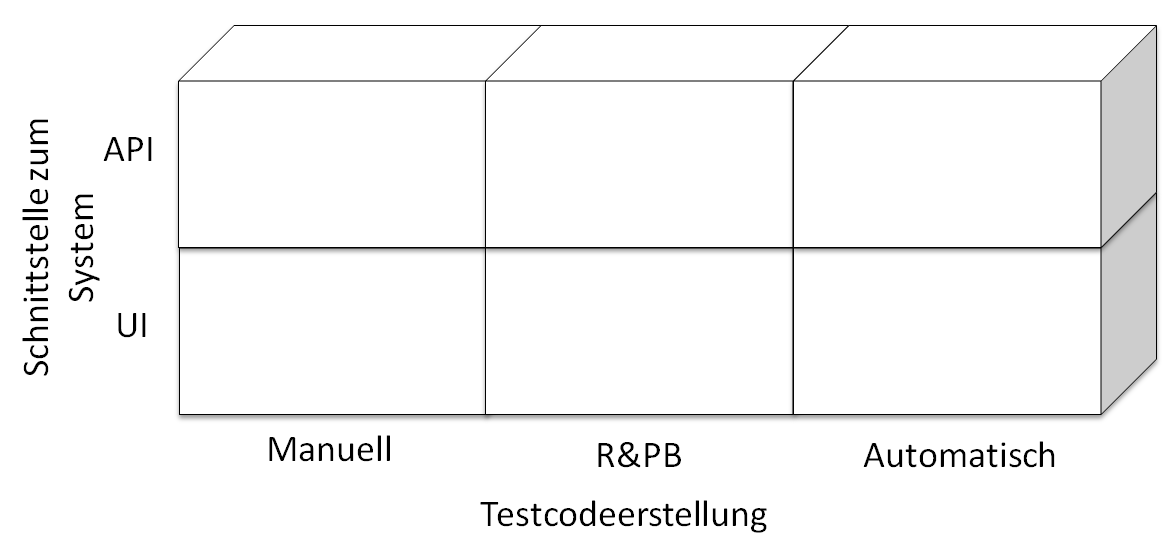
\includegraphics[scale=0.7]{img/bereicheTestcodeerstellung.png}\\
  \footnotesize\sffamily\textbf{Quelle:} vgl. \cite{meszaros_agile_2003}
  \caption{Verschiedene Möglichkeiten der Testcodeerstellung}
  \label{fig:bereicheTestcodeerstellung}
\end{figure}

Meszaros et al. \cite{meszaros_agile_2003} haben eine ähnliche Matrix aufgestellt, die noch um eine weitere Dimension der Testgranularität (Unit-, Integrations- und System-Test) erweitert ist. Diese Dimension hat allerdings nur wenig Auswirkung auf die Herangehensweise in der Testautomatisierung und wurde deshalb in Abbildung \ref{fig:bereicheTestcodeerstellung} nicht mit aufgeführt.
Im Folgenden wird, mit Hilfe von Beispielen, auf die Schnittstellen API und UI in Kombination mit der Manuellen- und R\&PB-Testcodeerstellung näher eingegangen.
Die vollautomatisierte Testcodeerstellung mittels modellbasierten Testen, dargestellt durch die beiden rechten Quader in Abbildung \ref{fig:bereicheTestcodeerstellung}, befindet sich außerhalb des Rahmens dieser Arbeit und wird daher nicht genauer betrachtet.

\subsubsection{API}
\label{subsubsec:API}

Unter der Abkürzung API sind in diesem Zusammenhang alle Schnittstellen zu verstehen, die intern von der zu testenden Anwendung angeboten werden. Darunter fällt beispielsweise das direkte aufrufen von Servicemethoden, die als Businesslogik innerhalb der Anwendung bereitgestellt werden.\\
Eine weit verbreitete Gruppe von Frameworks, welche oft diese Art der Schnittstelle verwenden, sind die modernen \grq XUnit-Frameworks\grq. In den meisten Programmiersprachen existiert ein Unit-Framework, mit dem es möglich ist, direkt die im Programm angebotene Logik mit automatisierten Testfällen zu überprüfen. In der Praxis wird diese Aufgabe meist direkt von einem Entwickler, in Form von Unit-Tests (Komponenten-Tests) übernommen. Der Begriff \grq XUnit-Frameworks\grq\ kann leicht missverstanden werden, da er impliziert, dass es sich bei den mit Hilfe des Frameworks umgesetzten Testfällen immer um Unit-Tests handelt. Es können jedoch Testfälle aller Teststufen, von Unit- bis System-Test, mit Hilfe dieser Frameworks umgesetzt werden.
Die Testcodeerstellung erfolgt dabei manuell, womit diese Art der Automatisierung ein Beispiel für den oberen linken Quader in Abbildung \ref{fig:bereicheTestcodeerstellung} darstellt.\\
Neben dem manuellen Vorgehen beschreiben Meszaros et al. \cite{meszaros_agile_2003} auch die Möglichkeit \grq record and playback\grq\ für Testfälle zu verwenden, die als Schnittstelle die API ansteuern.
Hierfür muss eine \grq record and playback\grq-Mechanismus auf API-Ebene für die zu testende Software entwickelt werden. Darüber ist es dann bei einem manuellem Testlauf möglich, all das aufzuzeichnen, was den Zustand des Systems beeinflusst hat. Aus diesen Aufzeichnungen kann dann Testcode erzeugt werden, der es ermöglicht die gewünschten Abläufe zu wiederholen. Solch ein Vorgehen wäre ein Beispiel für den oberen mittleren Quader in Abbildung \ref{fig:bereicheTestcodeerstellung}. Diese Art der Testcodeerstellung findet aber keine verbreitete Anwendung.

\subsubsection{UI}
\label{subsubsec:UI}
Bei Testfällen, die als Schnittstelle zum System das User-Interface verwenden, ist laut  Meszaros et al. \cite{meszaros_agile_2003} vor allem \grq record and playback\grq\ ein sehr weit verbreiteter Ansatz. Es existieren zahlreiche kommerzielle Testwerkzeuge, um dieses Vorgehen zu unterstützen, wie beispielsweise HP Unified Functional Testing \cite{hp_testautomatisierung_2015}, aber auch Open-Source-Lösungen wie Selenium \cite{selenium_selenium_2015}.\\
Diese Tools ermöglichen es Abläufe aufzuzeichnen, um sie später automatisch zu wiederholen. Die Testfälle werden dafür zunächst manuell auf der Benutzeroberfläche der Anwendung durchgeführt. Während dieser manuellen Testausführung können die vom Tester getätigten Eingaben vom Tool gespeichert werden. Die gespeicherten Interaktionen werden dann verwendet, um daraus Testcode zu generieren, mit dem die Abläufe auf der Benutzeroberfläche beliebig oft wiederholt werden können. Dieses Art der Testcodeerstellung wird in Abbildung \ref{fig:bereicheTestcodeerstellung}, durch den unteren mittleren Quader dargestellt.\\
Der untere linke Quader steht für manuell erstellten Testcode, der als Schnittstelle zum System das User-Interface verwendet. Oft handelt es sich dabei um Testfälle, die analog zu Abschnitt \ref{subsubsec:API} ein \grq XUnit-Frameworks\grq\ zur Testausführung verwenden. Diese Frameworks können um Aufsätze, wie beispielsweise HttpUnit \cite{httpunit_httpunit_2015} oder Selenium \cite{selenium_selenium_2015} erweitert werden. Mit Hilfe dieser Erweiterungen ist es möglich, Testfälle nicht mehr nur gegen die API der zu testenden Software zu entwickeln, sondern zur Steuerung die Benutzeroberfläche zu verwenden. Neben Aufsätzen für vorhandene Frameworks existieren auch zahlreiche eigenständige Tools, wie beispielsweise MicroFocus SilkTest \cite{silk_test_borland_2015}, welche neben Webanwendungen auch die Möglichkeit zum Testen von Desktopanwendungen bieten.\\
Testcode von Hand zu schreiben ist ein weit verbreitetes Vorgehen. Vor allem immer dann, wenn kein vorhandenes Testtool verwendet wird, sondern das Automatisierungsframework für die zu testende Software selbst entwickelt wurde.


\subsection{Testdurchführung}
\label{subsec:testdurchführung}
Unter Testdurchführung versteht man das Ausführen der Testfälle, sowie das Aufzeichnen von Testergebnissen bzw. Testausgaben. Nach den Erfahrungen von Amannejad et al. \cite{amannejad_search-based_2014} ist dieser Bereich der Testautomatisierung derjenige, der von den meisten Testern am engsten mit der Automatisierung verbunden wird.\\
Die Möglichkeit zur Automatisierung hängt in diesem Schritt stark von den gewählten Methoden in den vorangegangenen Phasen des Testprozesses ab. Oft ist eine automatisierte Testdurchführung bereits ohne zusätzlichen Aufwand möglich. Vor allem dann, wenn der Testcode zuvor Tool bzw. Framework unterstützt erstellt wurde.
Die meisten Tools und Frameworks ermöglichen bereits eine automatisierte Testdurchführung.\\
Im besonderen Maße sind an dieser Stelle, aufgrund ihrer hohen Verbreitung, erneut die \grq XUnit-Frameworks\grq\ zu nennen.
In Abschnitt \ref{subsec:testcodeerstellung} wurde aufgezeigt, dass diese Frameworks oft in der manuellen Testcodeerstellung verwendet werden. Das Unit-Framework übernimmt dabei die automatisierte Ausführung des Testcodes, sowie die Präsentation der Testergebnisse und ist damit ein Beispiel für ein Framework, welches die Testdurchführung automatisiert.\\
Probleme ergeben sich, wenn Testcode losgelöst von bereits vorhandenen Tools bzw. Frameworks entwickelt wurde. Der Testcode könnte beispielsweise gekapselt in Funktionen vorliegen und seine Ergebnisse in die Konsole loggen. Steigt die Anzahl der Testfälle, wird die Ausführung und vor allem die folgende Auswertung zum Problem. Der Aufwand, der später betrieben werden muss, um die Testfälle anhand ihrer Logmeldungen auszuwerten, kann so eine Dimension erreichen, die nicht mehr wirtschaftlich ist. Ein weiteres Problem stellt dar, dass eine gesonderte Ausführung von einzelnen Testfällen bzw. kleineren Testfallgruppen nur mit zusätzlichem Aufwand möglich ist.\\
Werden Testfälle daher ohne Tool- bzw. Framework-unterstützung erstellt, müssen zeitnah Überlegungen angestellt werden, wie diese einfach und auswertbar zur Ausführung gebracht werden können.
Diese Überlegungen resultieren meist in einem eigen entwickelten Testframework, welches die Ausführung des automatisierten Testcodes und die Aufzeichnung der Ergebnisse übernimmt.


\subsection{Testauswertung}
\label{subsec:testauswertung}
Nachdem die zu testende Software mittels eines Testfalls ausgeführt wurde, muss bestimmt werden, ob dieser erfolgreich oder fehlerhaft war. Diese Prüfung kann manuell erfolgen. Handelt es sich jedoch um automatisierte Testfälle, ist diese Prüfung meist über feste Akzeptanzkriterien direkt im Testfall hinterlegt. Im Fall von Testfällen, deren Durchführung über ein \grq XUnit-Frameworks\grq\ automatisiert wurde, werden Akzeptanzkriterien beispielsweise über sogenannte \grq Assertions\grq\ festgelegt.\\
Um die erwarteten Ergebnisse für einen Testfall zu finden, werden sogenannte Testorakel verwendet.
Jede Quelle, die Auskunft über ein zu erwartendes Ergebnis gibt, kann als Testorakel dienen.
Meist handelt es sich um Spezifikationen, die manuell ausgewertet werden.
Darüber hinaus gibt es aber auch zahlreiche Möglichkeiten und Versuche, diese zu automatisieren \cite{memon_automated_2000} \cite{richardson_specification-based_1992} \cite{shahamiri_comparative_2009}.
Automatisierte Testorakel können dann wiederum für die Auswertung der Testergebnisse dienen. Eine manuelle Auswertung kann so entfallen.\\
Bereits mit fest hinterlegten Akzeptanzkriterien, die manuell gefunden wurden, gilt laut Amannejad et al. \cite{amannejad_search-based_2014} die Testauswertung als automatisiert. Mittels automatisierter Testorakel kann diese jedoch noch ein höheres Level an Intelligenz erreichen. 




